\documentclass[final,12pt,twoside]{mcthesis}

\usepackage{pstricks}
\usepackage{epsf}
\usepackage{epsfig}
\usepackage{ulem}
\usepackage{hhline}
\usepackage{multirow}
\usepackage{amsmath}
\usepackage{amsfonts}
\usepackage{graphicx} 
\usepackage{fancyhdr}
\usepackage{float}
\usepackage{listings}
\usepackage{alltt}
\usepackage{amssymb}

\usepackage{glossary}
\renewcommand{\glossaryname}{Abbreviations}
\makeglossary

\begin{document}

\sloppy
\frontmatter
\thesistitle{State Diagrams: A New Visual Language For Programmable Logic Controllers}
\shorttitle{State Diagrams: a New Visual Language For PLC's}
\thesisauthor{FanFan Huang} 
\thesisdegree{M.A.Sc}
\thesisauthprevdeg{B.Eng}
\thesisauthprevdeguni{McMaster University}
\thesissupervisor{Dr. Martin von Mohrenschildt}
\thesisdate{\today}

\makepretitle
\maketitle

%list of custom definitions
\newcommand{\imgsmall}{100px}
\newcommand{\imgmedsmall}{120px}
\newcommand{\imgmed}{150px}
\newcommand{\imgsmlphoto}{175px}
\newcommand{\imgmedphoto}{200px}
\newcommand{\imgmedium}{300px}

\newcommand{\emphasize}[1]{\textit{#1}}
\newcommand{\plccharts}{\emphasize{Logic Control Chart} }
\newcommand{\plcchart}{Logic Control Chart}
\newcommand{\tablefontsize}{\tiny}

\newtheorem{definition}{Definition}[section]

%improve section numbering to include subsubsections
\setcounter{secnumdepth}{3}
\setcounter{tocdepth}{3}
%\dsp
\addcontentsline{toc}{chapter}{Abstract}
%abstract

Ladder logic has been the dominant defacto method for programming programmable logic controllers for over 30 years. Primarily designed as a replacement for electronic relay boxes ladder logic follows the analogies of circuits and wires. With the changes in education and training ladder logic has not kept up with the times. Ladder logic is difficult to understand for a software trained operator and with increasingly difficult control logic strategies ladder logic has become cumbersome and difficult to use.

This thesis seeks to examine a different approach to visual programming that is more suitable to modern software trained individuals. A visual programming language will be established based on finite state machines. We will then define both the syntax and semantics of our visual language, demonstrate the correctness of operation and execution. This thesis will also define a reference hardware platform and will define our graphical tool used to construct our programs.

The major contributions of this thesis include the development of a prototype programming language, a graphical integrated development environment tool, and a prototype hardware environment.
\newpage
%\addcontentsline{toc}{chapter}{Acknowledgements}
%TODO: ACK need acknowledge!!!




\tableofcontents
\listoftables
\listoffigures

\label{pre end}
\mainmatter

\addcontentsline{toc}{chapter}{Abbreviations}
\printglossary


\chapter{Preface}

\section{Structure of this Thesis}

\noindent
Chapter 2: \emphasize{Overview of Existing Technology}. We will begin by introducing the reader to existing PLC\glossary{name={PLC}, description={Programmable Logic Controller}} implementations. We will go into the history behind programmable logic controllers and their usages. We will also give the user an idea of what kinds of modules manufacturers have created in the industry over time.
\\

\noindent
Chapter 3: \emphasize{Introduction To Ladder Logic}. In this chapter we will expose the reader to the existing language (Ladder Logic) that is currently in use in the industry. The reader will be exposed to the syntax and semantics of this language. In addition the user will also obtain some background insight as to how the language came into looking as it does today.
\\

\noindent
Chapter 4: \emphasize{Software}. The software section covers all of the software implementation information of the proposed language Logic Control Chart\glossary{name={LLC},description={Logic Control Chart}}. We begin by defining the goals in constructing LLC\glossary{name={LLC},description={Logic Control Chart}}. Next the language is then defined for LLC. In the final two sections we go into implementation details of the software package as well as show correctness of the diagram to code translation.
\\

\noindent
Chapter 5: \emphasize{Hardware}. In this section we go into detail about the hardware reference platform. We introduce the hardware framework which allows multiple microcontrollers to be utilized. We finish by showing parts of the hardware driver code that must be implemented should the reader wish to implement their own hardware board.
\\

\noindent
Chapter 6: \emphasize{Summary}. This chapter presents all the conclusions of the work. In addition we also recommend future directions this thesis can go if continued.
\\

\noindent
Appendix: Contains examples and diagrams in Ladder Logic.

%Overview of existing technology (hardware)

\chapter{Overview of Existing Technology}
\section{PLC Hardware Controller Implementations}
%link to automotive statement: http://www.amci.com/tutorials/tutorials-what-is-programmable-logic-controller.asp
Programmable Logic Controllers (PLC) have been around for over 30 years and as such there have been many iterations and designs. The original Programmable Logic Controllers came into being to fill the need of automotive manufacturers replacing traditional relays with digital control. To this day modern PLC's still use graphical analogies of circuits and relays in order to construct their programmable logic.

Mitsubishi Automation, Siemens, and Omron are just a few of the big producers of industry standard PLC's although the shape and form factor differ between manufacturers differ PLC's always consist of 3 distinct parts.  The input module, the main controller unit and the output module. This separation exists due to varying requirements for analog inputs and different output level requirements in order to drive heavy machinery. I/O modules may consist of thermo sensors, ambient light sensors, resistive sensors, or a direct connection the the external circuitry. Likewise the output module may also be composed of both analog or digital output pins.

%source http://www.sea.siemens.com/step/templates/lesson.mason?plcs:2:3:1
Programs are executed from the main PLC control unit. An iteration of execution is refered to as a scan. A scan is broken up into 4 phases: Self-Test, Input scan, Logic solve / scan, and Output scan. In detail each phase and their specific jobs are:

\begin{itemize}
	\item\textbf{Self-Test:} All PLC's contain self diagnostic routines, this includes communication checks between the main control unit and the I/O modules. If a fault is found it is handled here before any of the execution is allowed to proceed.
	\item\textbf{Input Scan:} All inputs both from the input modules and from the internal memory are scaned. This is done in a single step to make sure that all future calculations for the currently executing scan has consistent data. You may note that updates are not read until the next input scan.
	\item\textbf{Logic Solve / Scan:} Calculations and computations from the user programs are computed in this step if values are to be stored back into internal registers they are now put into temporary registers. Similarily if external output is required it is written to a temporary internal register that will hold the output until the output phase is executed.
	\item\textbf{Output Scan:} Internal temporary registers are written to their destination registers in one step. External outputs take on the values held by the registers that stored data for the output modules all outputs also take place in one step.
\end{itemize}

Each of these phases semantically can be assumed to execute cocurrently thus, the order of individual instructions in each phase is of no consequence. This closely follows the Ladder Logic (please see section \ref{section:ladderlogic}) in that the entire program executes cocurrently on multiple rungs. Internally however PLC's do have a sequential deterministic order in which instructions are executed, this is a side effect of using microcontrollers in the main control unit. In this way it can be said that each phase is considered concurrent if we consider a cycle time greater than the time it takes to execute the last instruction. If an external device takes samples at this rate it is irrelevent from its perspective that the processing is not actually happening cocurrently to the observing device the two behaviors are equivalent.

The input and output modules generally connect to the main module via serial links however some companies also include network commuication over standard shielded ethernet\cite{rockwell_io,rockwell_tech_pub}. Generally serial communication is used more often when the input and output modules are at a close distance to the controller unit such as in a modular PLC design. The network interface on the other hand is used when the input or output module needs to be located far away from the main controller unit\cite{rockwell_tech_pub} as is often the case in automated production facilities.

Programmable logic controllers can classified into three categories: Integrated, Modular, and Large Scale automation. The integrated category includes small one board solutions generally better suited for low power or embedded applications. The modular category consists of PLC's that have a rack that houses the power supply, and several modular slots for both the microcontroller and the input output modules.



%introduction to ladder logic

\chapter{Introduction to Ladder Logic}
\section{Background of Ladder Logic}
\label{section:ladderlogic}

%docment link: http://www.plcs.net/chapters/whatis1.htm
%reasons for development
Ladder logic was originally developed to replace physical relays in PLC's.
As a result the ``language'' resembles a circuit diagram. The left most
and right most ``rung'' represent power rails analogous to GND and VCC what's
placed in between those rungs is the load components/cite{ebookmorris}. In 
the case of programming the entire logic is created from loads you place 
inside these power rails. 

Several other conventions are also observed, power always flows from left 
to right along each rung. Power also flows from top to bottom along the 
rails. This is counter intuitive since ladder logic is suppose to be 
analogous to a circuit schematic and there is no implicit
ordering in circuits. In addition each run must start with inputs and end
with at least one output. Any device that is on a rung is shown in its
initial position.

Modern PLC's operate more like a traditional micro controller and thus the 
original schematic based language can prove to be awkward to work with.

The inputs in ladder are referred to as a load and represented by the 
symbol $-\vert ~ ~ \vert-$. %need reference from tutorial
Loads are boolean values and can be a negated input using the $-\vert/\vert-$ symbol. 
In addition an address is usually assigned to each input referring to 
which port on the physical PLC the input is connected to. Logical and 
can be formed by having two logical loads on one rung \cite{ebookmorris}. 
Similarly logical or can be formed by creating a branch along one 
rung as shown in figure. %figure # %refer to figure here

We can define the language of Ladder Logic as follows $Q = \langle M,S,C,F,R,P \rangle $

\begin{itemize}
	\item M: set of monitored variables.
	\item S: set of state variables.
	\item C: set of controlled outputs.i
	\item R: set of rungs.
	\item P: set of power rails.
\end{itemize}

\begin{figure}[htp]
    \centering
    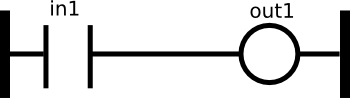
\includegraphics[width=\imgsmall]{./images/intro_fig1.png}
    \caption{Basic Ladder Logic Diagram}
    \label{fig:intro_fig1}
\end{figure}

The most basic structure of ladder logic is shown in figure \ref{fig:intro_fig1}. 
We have 
$$M=\lbrace in_1 \rbrace, S=\lbrace out_1 \rbrace, C=\lbrace out_1 \rbrace, R=\lbrace rung_1 \rbrace, P=\lbrace L,R \rbrace.$$
Note that $rung_1$ is not explicitly labelled in ladder logic but we give it a name here
so we may demonstrate our language framework.

The semantics of figure \ref{fig:intro_fig1} is then: 
\begin{table}[htp]
    \centering
    \begin{tabular}{|l|l|l|}
        \hline
        Action & Result \\
        \hline
        $@T(in_1 = true)$ & $out_1 := true$ \\
        \hline
        $@T(in_1 = false)$ & $out_1 := false$ \\
        \hline
    \end{tabular}
    \caption{Semantics for Fig \ref{fig:intro_fig1}}
    \label{table:table_for_fig1}
\end{table}


Where $@T(<condition>)$ is used to denote the positive edge of a condition becoming true.
We also assume negligible delay between the action occurring and the result being asserted.
It is important to note that our function table must be complete that is have an entry for
all possible combinations in the input domain.

\begin{figure}[htp]
    \centering
    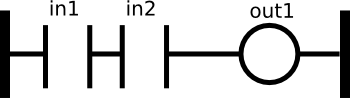
\includegraphics[width=\imgsmall]{./images/intro_fig2.png}
    \caption{Simple AND Logic Diagram}
    \label{fig:intro_fig2}
\end{figure}

When multiple actions are connected on the same rung it is interpreted as a logical AND 
expression. In figure \ref{fig:intro_fig2} we can expand our model to:

$$M=\lbrace in_1, in_2 \rbrace, S=\lbrace out_1 \rbrace, C=\lbrace out_1 \rbrace, R=\lbrace rung_1 \rbrace, P=\lbrace L,R \rbrace.$$

We can see that both $in_1$ and $in_2$ are on $rung_1$. This is interpreted as follows:

\begin{table}[htp]
    \centering
       \begin{tabular}{|l|l|l|}
        \hline
        Action & Result \\
        \hline
        $Initial$ & $in_1 := false, in_2 := false, out_1 := false$\\
        \hline
        $@T(in_1 = true \wedge in_2 = true)$ & $out_1 := true$ \\
        \hline
        $@T(in_1 = false \vee in_2 = false)$ & $out_1 := false$ \\
        \hline
    \end{tabular}
    \caption{Semantics for Fig \ref{fig:intro_fig2}}
    \label{table:table_for_fig2}
\end{table}

The conditions $in_1$ and $in_2$ are combined to form our composed action $@T(in_1 = true \wedge in_2 = true)$ 
as seen in table \ref{table:table_for_fig2}. We also note that there is no action for each individual condition
becoming true nor do we need to individually calculate the timing on $in_1$ or $in_2$ individually.

\begin{figure}[htp]
    \centering
    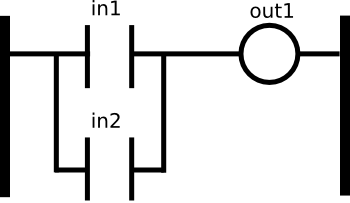
\includegraphics[width=\imgsmall]{./images/intro_fig3.png}
    \caption{Branching Rungs}
    \label{fig:intro_fig3}
\end{figure}


In addition to multiple actions connected to the same rung, actions can also be branched. A branched rung as
show in figure \ref{fig:intro_fig3} behaves like a logical OR. In addition two or more rungs can be joined
as show in figure \ref{fig:intro_fig3a}. The semantics are equivalent in both figure \ref{fig:intro_fig3} and 
figure \ref{fig:intro_fig3a}.

\begin{figure}[htp]
    \centering
    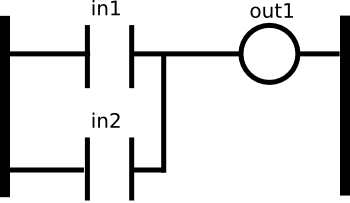
\includegraphics[width=\imgsmall]{./images/intro_fig3a.png}
    \caption{Branching Rungs (Alternative)}
    \label{fig:intro_fig3a}
\end{figure}

\begin{table}[htp]
    \centering
       \begin{tabular}{|l|l|l|}
        \hline
        Action & Result \\
        \hline
        $Initial$ & $in_1 := false, in_2 := false, out_1 := false$\\
        \hline
        $@T_n(in_1 = true \vee in_2 = true)$ & $out_1 := true$ \\
        \hline
        $@T_n(in_1 = false \wedge in_2 = false)$ & $out_1 := false$\\
        \hline
    \end{tabular}
    \caption{Semantics for Fig \ref{fig:intro_fig3} and Fig \ref{fig:intro_fig3a}}
    \label{table:table_for_fig3}
\end{table}

Since the semantics are the same for both figure \ref{fig:intro_fig3} and figure \ref{fig:intro_fig3a} we can
express both outcomes with function table \ref{table:table_for_fig3}.
As before in table \ref{table:table_for_fig2} in table \ref{table:table_for_fig3} $in_1$ and $in_2$ are composed to form our composed action $@T(in_1 = true \vee in_2 = true)$. However it is also possible to represent this action another way.

\begin{table}[htp]
    \centering
       \begin{tabular}{|l|l|l|}
        \hline
        Action & Result \\
        \hline
        $Initial$ &$in_1 := false, in_2 := false, out_1 := false$\\
        \hline
        $@T(in_1 = true)$ & $out_1 := true$ \\
        \hline
        $@T(in_2 = true)$ & $out_1 := true$ \\
        \hline
        $@T(in_1 = false \wedge in_2 = false)$ & $out_1 := false$\\
        \hline
    \end{tabular}
    \caption{Semantics for Fig \ref{fig:intro_fig3} and Fig \ref{fig:intro_fig3a}}
    \label{table:table_for_fig3a}
\end{table}

In table \ref{table:table_for_fig3a} we choose to represent $in_1$ and $in_2$ as separate actions. This matches figure
\ref{fig:intro_fig3a} more closely but also makes any verification harder than table \ref{table:table_for_fig3}. For
smaller examples table \ref{table:table_for_fig3} make more sense since you can verify relatively simple smaller functions
quite fast. If a system becomes reasonably large however there might be motivation to use the style shown in 
table \ref{table:table_for_fig3a} since it will allow more complex functions to be decomposed into simpler actions.
Since semantically the two are equivalent this paper will focus to the first convention.




%not sure if I should put rung definition here
\pagebreak[4]

\begin{figure}[htp]
    \centering
    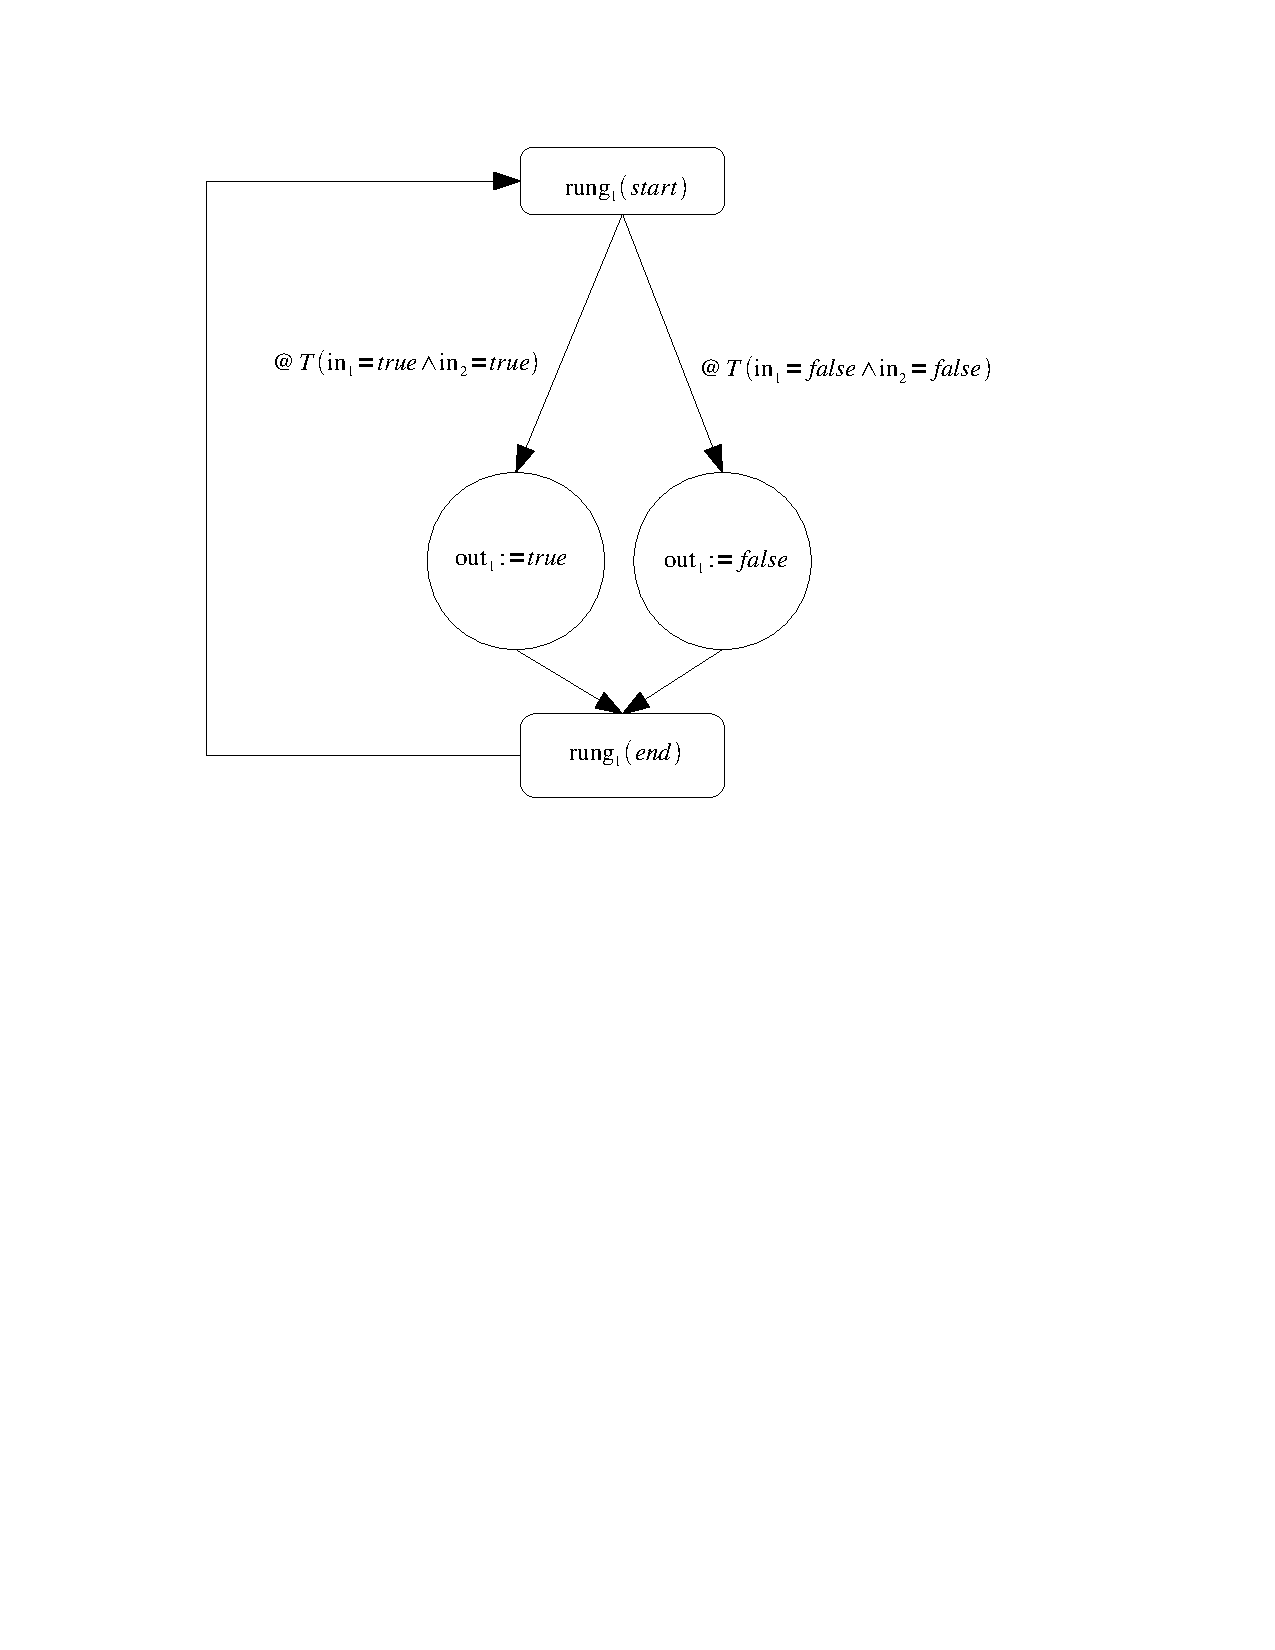
\includegraphics[trim= 0 140mm 40mm 10mm, clip, width=\imgmed]{./images/intro_and_graph.pdf} %custom size
    \caption{State chart conversion for table \ref{table:table_for_fig2}}
    \label{fig:intro_and_graph}
\end{figure}

A rung can be defined as a directed acyclic graph with exactly one source and one sink. The state variables form guard conditions along the edges. A branch in this case represents 2 edges leaving one node. For example figure \ref{fig:intro_fig2}
can be easily converted into a state chart by observing the results in table \ref{table:table_for_fig2}. 
Each row of table \ref{table:table_for_fig2} is directly converted into an edge with the appropriate guard conditions.
Each output assertion is given their own state. Finally in figure \ref{fig:intro_and_graph} we observe 1 source for the
graph being the start state of the rung, and one sink for the graph being the end state for the rung. We can equivalently take figure \ref{fig:intro_fig3} observe its function table \ref{table:table_for_fig3} and produce an equivalent state chart from its function table.

\pagebreak[3]

\begin{figure}[htp]
    \centering
    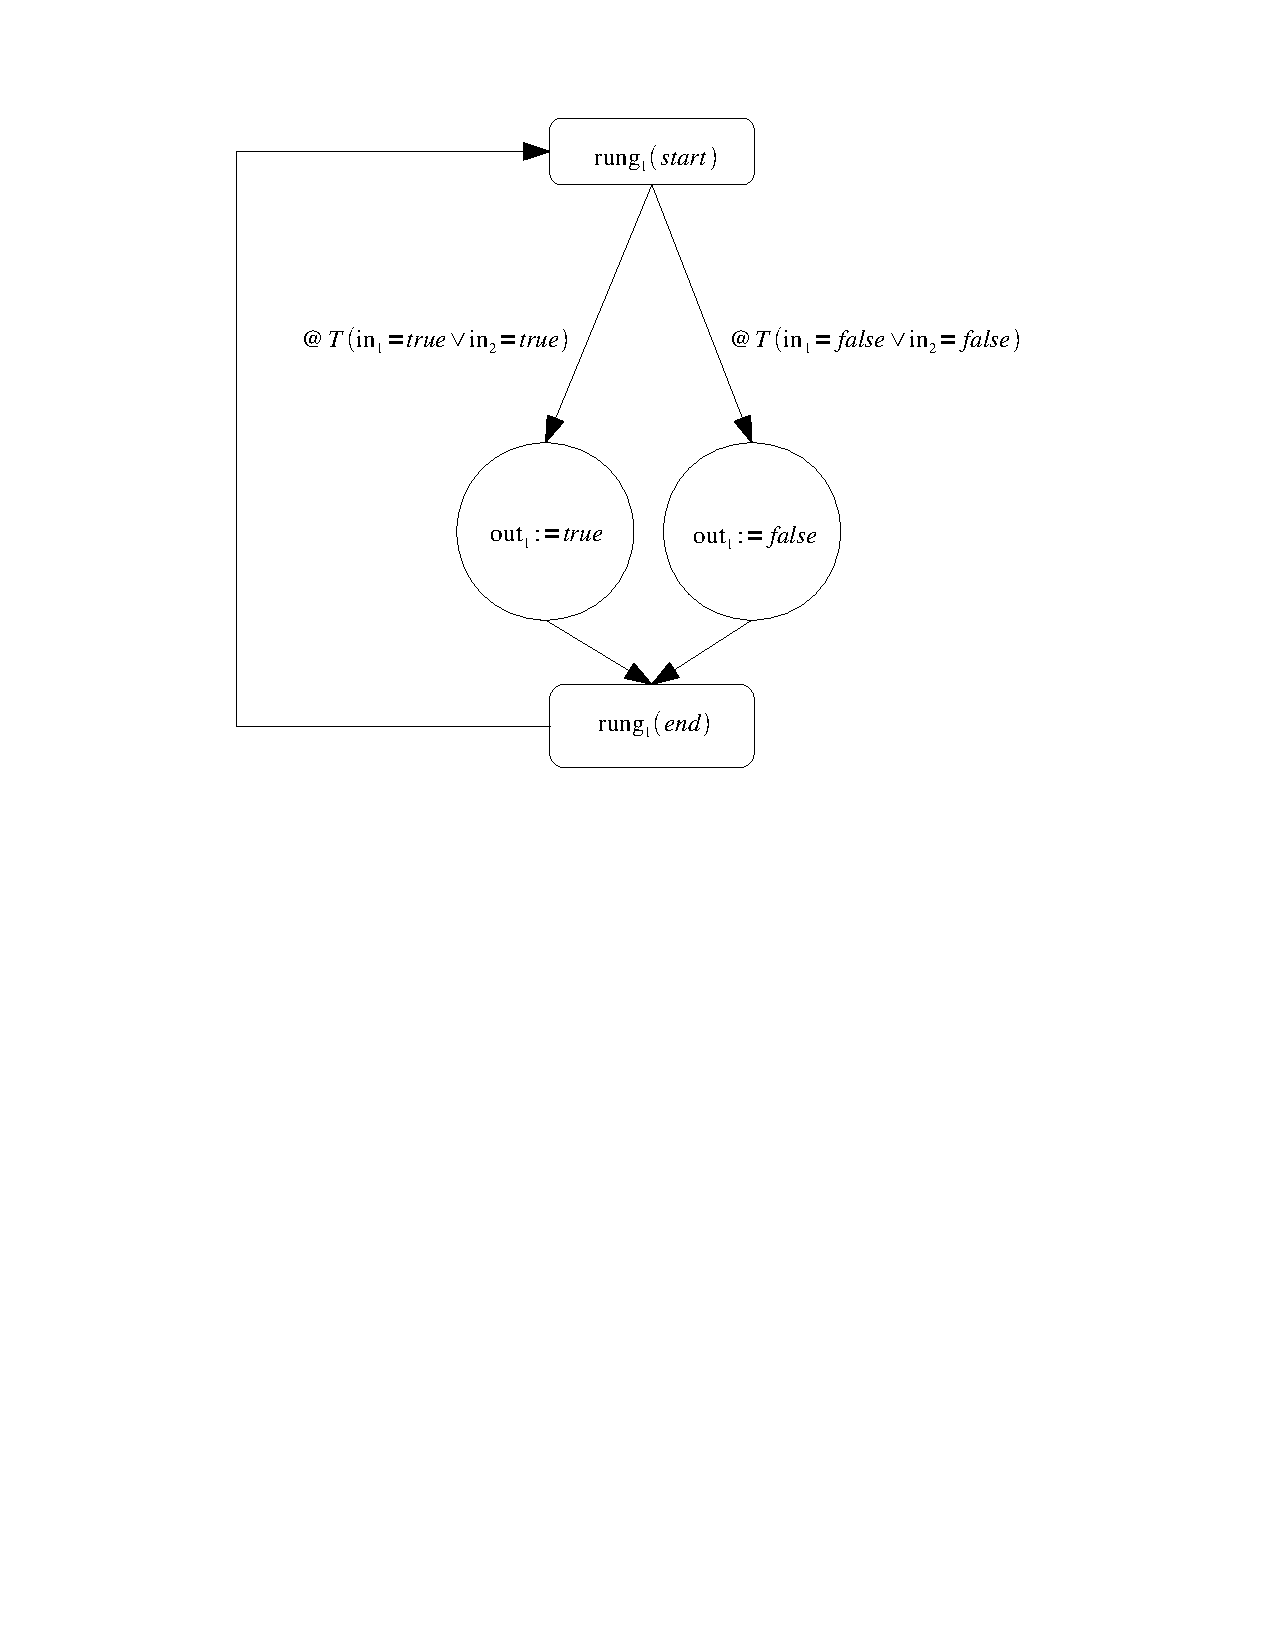
\includegraphics[trim= 00mm 140mm 40mm 10mm, clip, width=\imgmed]{./images/intro_or_graph.pdf} %custom size
    \caption{State chart conversion for table \ref{table:table_for_fig3}}
    \label{fig:intro_or_graph}
\end{figure}

Thus, each rung can be converted into an equivalent state chart by examining its 
function table, assigning the state variables to guard conditions, and creating a
state for each of the outputs. For completeness we complete this procedure to produce
a state chart equivalent representation for figure \ref{fig:intro_fig3a} and its
corresponding table \ref{table:table_for_fig3a}.


\begin{figure}[htp]
    \centering
    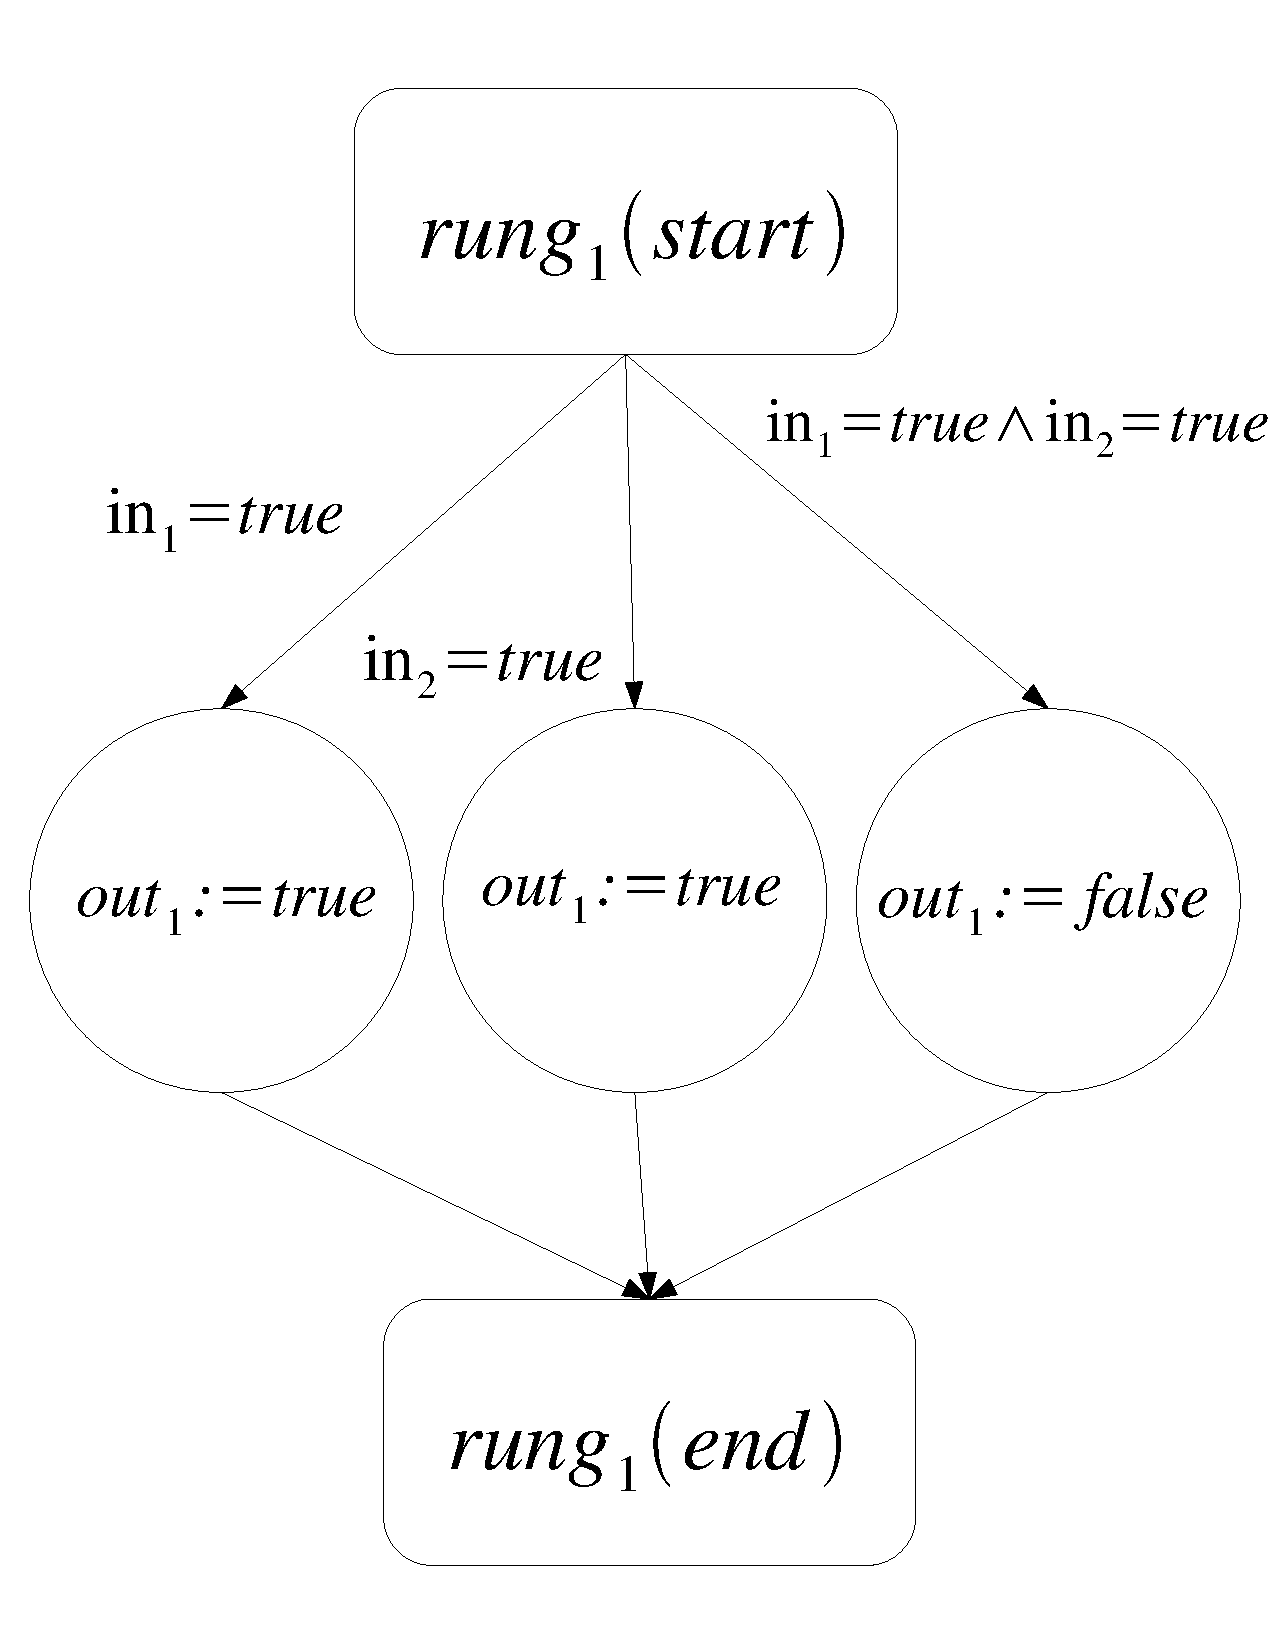
\includegraphics[width=\imgmedsmall]{./images/intro_or_graph_3a.pdf} %custom size
    \caption{State chart conversion for table \ref{table:table_for_fig3a}}
    \label{fig:intro_or_graph_3a}
\end{figure}

So far we've been looking at logic that has things happening instantaneously however ladder logic does contain methods for expressing more advance behaviour. Suppose you have a light that you want to be able to turn on and stay on after you push a button. With any of the ladder diagrams shown above the light would go out as soon as the buttons were all released. In order to keep the light on and constantly on after the button is pressed we introduce the concept of a latch. We modify our diagram shown in figure \ref{fig:intro_fig3a} making the output feed back into one of the inputs to our OR circuit. The result is show in figure \ref{fig:intro_fig_latched}.

%figure for latched circuits 
\begin{figure}[htp]
    \centering
    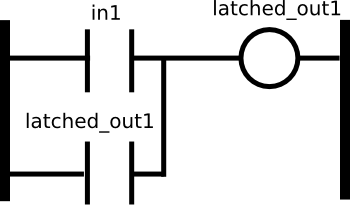
\includegraphics[width=\imgsmall]{./images/intro_fig_latched.png} 
    \caption{Latched ladder logic circuit.}
    \label{fig:intro_fig_latched}
\end{figure}

The latched circuit operates the same way as the behaviour show in \ref{table:table_for_fig3a} the key difference is the feedback of the OR circuit replaces the second row of the function table.


\chapter{Software}
\label{ch:software}

%goals of this project
\section{Goals}

This project aims to improve on current industrial programmable logic controllers by introducing a more natural graphical programming method. In addition we will evaluate how to create a cost effective alternative using off the shelf parts to construct our own hardware PLC. In the process we aim to produce a final prototype that will have the same basic feature set of modern PLC's. This includes a main controller unit, with input and output capabilities, and a prototype of a basic IDE that will work in our new visual language. In this project we propose state machine diagrams as the method of choice. As state machines can be used to represent all current programming languages. It is also important for this project to understand the deficiencies of Ladder Logic (the current method). In addition we will evaluate the original use of PLC's and if the old methodologies are still applicable to their modern application. This analysis will provide further understanding on how the original programming methods have been outpaced by more recent technology.

Due to the scope of this project we must deliver several components in order to achieve an acceptable proof of concept. The components and their sub-goals are as follows:

We must deliver a main controller unit with an on-board embedded OS. This main controller will serve as our CPU and will include the input and output units in addition to running our program. The main controller must be able to execute adequately fast in order to compete against commercial PLC's. Since the user is not concerned with the execution speed of each instruction, fast refers to the time it takes for an input to trigger an output. We hope to utilize cheaper hardware but still equivalent speeds by allowing the user to specify instructions more closer to the actual chip supported instructions. This reduces the actual number of pseudo instructions required to perform a task. Our hardware will aim to not require executing in scans (see Figure \ref{fig:plcexecution}) and in doing so we hope to make better use of available hardware.

We must also design and formalize a visual programming language to be used as a replacement for Ladder Logic. This language will require precise definitions on how to interpret diagram elements. The language should also be designed to be easily understandable and generate efficient code. It should also be advanced enough to construct basic control programs. To practically utilize this language we will deliver a proof of concept IDE that will allow the user to enter programs using the visual programming language instead of Ladder Logic. This new IDE should work like a flow chart drawing program allowing the user to add and remove logic blocks at will. We aim to make this interface as intuitive as possible and also provide a fast efficient translation into machine code. In addition a simulator is also required to help developers visualize a program's execution. The simulator should contain basic step features to allow the programmer to step through each transition, and allow the developer to examine the contents of the variables in memory. The main goal of the IDE will be to provide an easy to understand visual environment where the user may enter their program and to minimize error where possible.

The final layer that will be added is a software to hardware compiler that will take user generated programs from the IDE and produce actual machine code. This will be achieved in two parts. First the IDE will compile the diagram into intermediate code. This intermediate code will be code that will stay hardware neutral and will resemble C. The intermediate code will contain many calls to functions that will be supported on the chip. These functions will be part of our hardware framework that will take the calls placed by intermediate language and translate them into hardware specific calls. From this design choice hardware specific code will stay on the hardware portion of this project and compiled software will stay hardware independent with specific support implemented by the hardware framework.

By delivering an initial proof of concept software and hardware system this project would allow for further development for modernizing programmable logic controllers. In addition it may also serve as a practical example of visual programming languages that are used to program embedded devices.

\newpage
%Introduction to state charts
\section{State Charts}

Our proposed visual programming language involves using directed state charts with guarded edges. Our languages differs in a few concepts from the usual state charts syntax in order to support features of the hardware. To better understand these differences we will first introduce all the syntax and semantics of a standard UML based state chart.

A State chart is generally defined as a diagram describing the behaviour of a discrete system. Such systems can be either finite state machines, or more complex systems abstracted to resemble a finite state machine. 

%http://en.wikipedia.org/wiki/State_diagram (find different source Taylor atomata paper
Mathematically a state chart can be defined as $M = \lbrace Q, \Sigma, Z, \delta, q_0, F \rbrace$

\begin{itemize}
	\item \textbf{Q:} Set of states.
	\item \textbf{$\Sigma$:} Set of input symbols or actions, these are used when checking guard conditions.
	\item \textbf{Z:} Set of output symbols generated by the system.
	\item \textbf{$\delta$:} Set of state transitions with the mapping $\omega: \Sigma \times Q \rightarrow Z$. These are drawn as arrows and are immediately taken if their guard conditions are true.
	\item \textbf{$q_0$:} Starting state, can be defined as an initial state with no incomming transitions.
	\item \textbf{F:} Accepting states for the system, can also sometimes represent the final state. Drawn as a double outline to the state symbol.
\end{itemize}

A state can be thought of as a set of operating conditions that for example in figure %\ref{fig:state_blink_light}
one such state the light is on.

%digram simple state transition for a blinking light {fig:state_blink_light}

We observe that transitions must always be connected on the tail end and the tip to a state. In addition if a transition can be taken it must be taken immediately. Transitions may also have a guard condition accociated with them. If a guard condition does not exist then it is assumed the transition can always be taken. In addition to a guard condition each transition may have an output accociated with them. Moore style state machines do not contain outputs on transition edges, Mealy machines do contain an extra output per transition.

%diagram for Moore + Mealy state machines

There are several ways a starting state can be defined as seen in figure {TODO: FIGURE REF}.%\ref{fig:state_moore_mealy}
One such way is to draw a edge that has no state connected to its tail, this generally looks like an edge out of nowhere. In our system we choose to use the UML symbol where the start state edge has a solid dot connected to the tail as shown in figure {TODO: FIGURE REF}. %\ref{fig:state_blink_light} // or other uml symbol

The accepting state is defined in state charts as any states where inputs are accepted. In other words this is generally a state in which the machine has successfully performed its task and is now ready to take on another one. Accepting states generally can reach all other states in the system. For our implimentation we do not need to model this behavior and therefor the concept of accepting states have been left out for practical purposes.

In a standard state chart a lot of implementation details can be hidden away and the diagram can be rather simple. In this example we see that there's no mention of how to turn on the light or turn off the light. Nor do we care if the light is connected to a particular port.

%Source wikipedia
TODO: The tyoe if state charts that we are using is a DIRECTED GRAPH with GUARDED EDGES. We have a starting state but not necessarily an ACCEPTING state.

TODO: Our state chart is very similar to an UML state diagram.

TODO: We might consider adapting our state chart to resemble UML digrams but that bit is under consideration. currently it does look very similar but edges do not have the correct formatting for guarded conditions on UML.

TODO: Minor detail, all of our states have an implicit edge going to END and will be used if no other conditions are true. We might consider showing the difference in the two.

TODO: Programming side, we need to enable saving because it's becoming a pain in the -bleep-.
   

\newpage
%Semantics of state charts
\section{Semantics of The State Chart Language}

The semantics used for our project was purposely modelled after UML2. As discussed in section \ref{sec:overviewstatechart} UML2 is essentially standard state charts with extensions added on to describe behaviours in states. The motivation to using UML2 as a basis for our state chart system consists of three primary details. First UML2 is quite well known and popular, this improves the potential acceptance of our tool. Secondly UML2 state chart syntax is more concrete than the other forms of state charts, giving a strong basis to construct our language around. Finally UML2 has the concept of internal activity or internal execution necessary for modelling the behaviour of an actual useful program.

The semantics of our state charts can be expressed mathematically as follows:

\begin{itemize}
	\item \textbf{Q:} A set of states.
	\item \textbf{$\Sigma$:} A set of assignments. $Q \times (v_0,v_1 \in \Sigma \bullet v_0 := v_1)$
	\item \textbf{$\tau$:} A set of transitions. $Q \times E \rightarrow Q$
	\item \textbf{$q_0$:} An initial starting state.
\end{itemize}

The set of states denoted by Q includes the starting state that is $(q_0 \in Q)$. Assignments in our system happen in sequence rather than all at once this method was chosen to allow sequential forumlae to be computed in our system easily. Assignments can be in the form of a constant or an equation. If a series of assignment were found in a single state as follows:

\begin{align}
v_1 := v_0 \label{eqn:assign0} \\ 
v_0 := v_1 \label{eqn:assign1}
\end{align}

We would see that the result $v_1 = v_0$ it is important to note this since generally in state charts it is understood that assignments happen cocurrently in such a case equations \ref{eqn:assign0} and \ref{eqn:assign1} would produce a swap where $v'_1 = 'v_0$ and $v'_0 = 'v_1$. In normal state charts we read assignments such as in equations \ref{eqn:assign0} and \ref{eqn:assign1} as these assignments will take place upon entry of the state. For our semantics however, we read them in a sequential fashion for example: Upon entry of the state, first equation \ref{eqn:assign0} is assigned, then \ref{eqn:assign1} right afterwards.

\begin{figure}[htp]
    \centering
    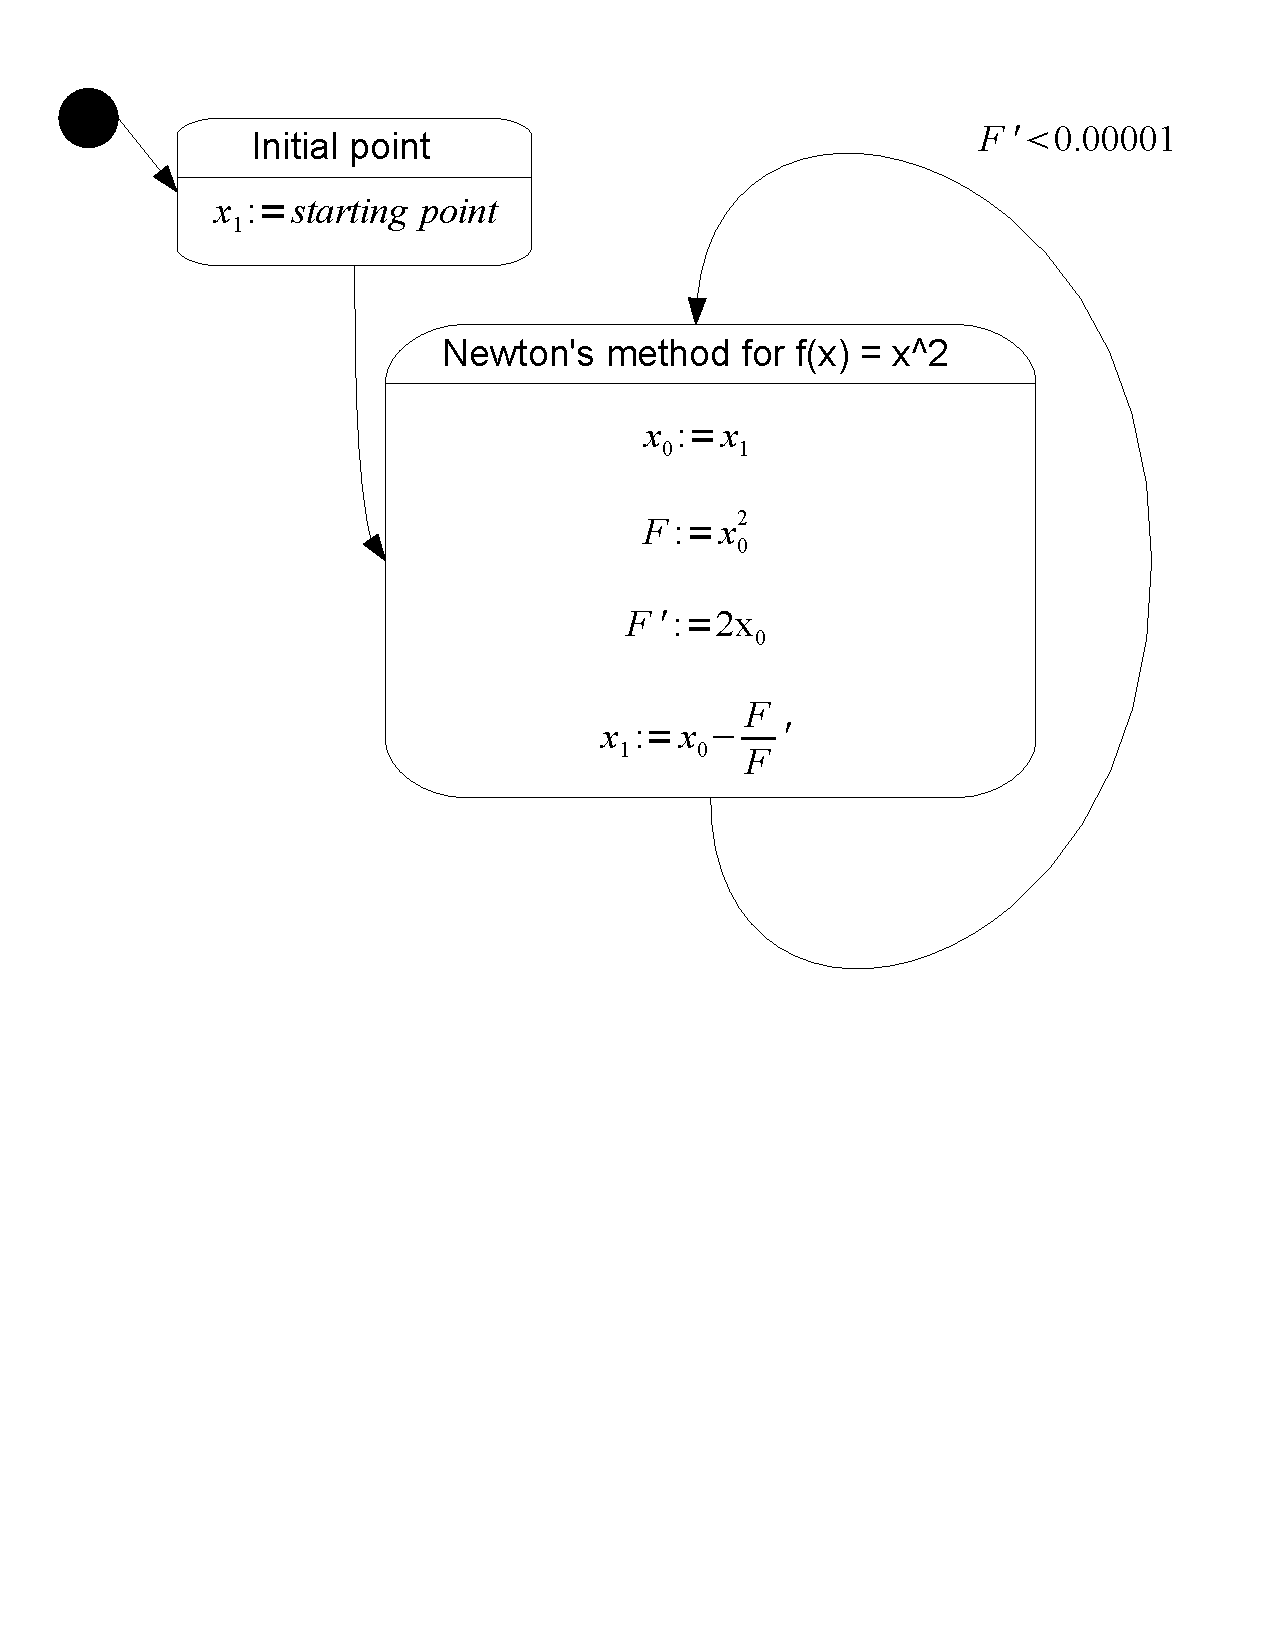
\includegraphics[trim= 10mm 110mm 10mm 10mm, clip, width=\imgmedium]{./images/state_uml2_newtons.pdf}
    \caption{Newton's Method Approximation}
    \label{fig:state_uml2_newtons}
\end{figure}

The advantage of sequential assignments over cocurrent assignments can be seen when trying to compute more complicated formulas as seen in figure \ref{fig:state_uml2_newtons}. Figure \ref{fig:state_uml2_newtons} computes the newton's approximation of $x^2$ given a starting point. If the same formula was to be computed with cocurrent assignments many more states would be required. Thus although this choice slightly deviates from UML2 state charts it was decided the benefits to usability was too great to strictly adhere to the UML2 semantics.

\begin{figure}[htp]
    \centering
    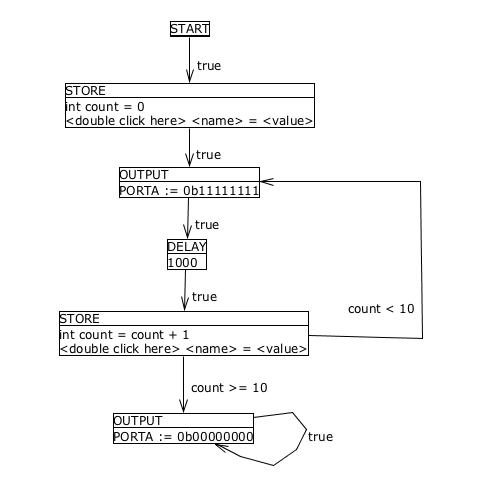
\includegraphics[width=230px]{./images/tool_transition_example.png}
    \caption{PLC Edit Example}
    \label{fig:tool_transition_example}
\end{figure}

\begin{figure}[htp]
    \centering
    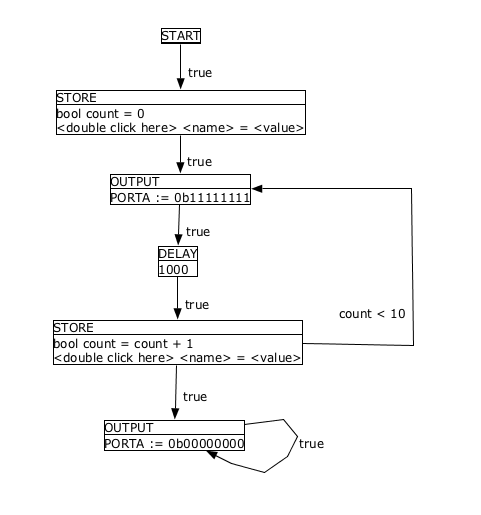
\includegraphics[width=230px]{./images/tool_transition_example_bad.png}
    \caption{PLC Edit Example With Bad Transitions}
    \label{fig:tool_transition_example_bad}
\end{figure}

Transitions in the language must be mutually exclusive that is if it is invalid to have two transitions that can both be taken at any point. Figure \ref{fig:tool_transition_example} shows an example of this done correctly the two guard conditions "count < 10" and "count >= 10" ensure mutal exclusivity. When mutual exclusion is not ensured such as in figure \ref{fig:tool_transition_example_bad} the language is undefined. The state chart language currently does not allow for cocurrent execution. Therefore our language this would be seen as an ambiguity and the outcome (as in which edge would be taken) is undefined.        

\newpage
%State Digram Syntax
\section{Syntax of \plcchart}
\label{sec:statechartsyn}

Abstract syntax of \plcchart language:
\begin{definition}
\plcchart

\begin{itemize}
	\item Eq := $\;$ \boldmath$=$\unboldmath $\; \mid \;$ \boldmath$\neq$\unboldmath $\; \mid \;$ \boldmath$<$\unboldmath $\; \mid \;$ \boldmath$\leq$\unboldmath $\; \mid \;$ \boldmath$>$\unboldmath $\; \mid \;$ \boldmath$\geq$\unboldmath	
	\item Op := $\;$ \boldmath$+$\unboldmath $\; \mid \;$ \boldmath$-$\unboldmath $\; \mid \;$ \boldmath$*$\unboldmath $\; \mid \;$ \boldmath$/$\unboldmath $\; \mid \;$ \boldmath$\%$\unboldmath $\; \mid \;$ \boldmath$\&\&$\unboldmath $\; \mid \;$ \textbf{\texttt{||}} $\; \mid \;$ \boldmath$\mathbin{\char`\^}$\unboldmath

	\item Expression := Expression Op Expression $\mid$ Op Expression $\mid$ Variable $\mid$ \textbf{Constant}
	
	\item Type := \textbf{Char} $\mid$ \textbf{Int} $\mid$ \textbf{Long} $\mid$ \textbf{Bool} $\mid$ \textbf{Float}
	\item Variable := $[A-Za-z]^+[A-Za-z0-9]^*$

	\item Condition := Expression Eq Expression $\mid$ Variable

		
	\item StoreBlock := Type Variable = Expression $\mid$ Type Variable = Expresion; StoreBlock
	\item DelayBlock := Expression
	\item OutputBlock := \textbf{PORTOUT} = Variable
	\item InputBlock := Type Variable = \textbf{PORTIN}
	\item Block := StoreBlock $\mid$ OutputBlock $\mid$ DelayBlock $\mid$ InputBlock

	
	\item Transition := Block Condition Block $\mid$ Block Condition Transition
	
	\item Program := \textbf{StartBlock} $\mid$ \textbf{StartBlock} Condition Block $\mid$ \textbf{StartBlock} Condition Transition
\end{itemize}
\end{definition}

\begin{figure}[htp]
    \centering
    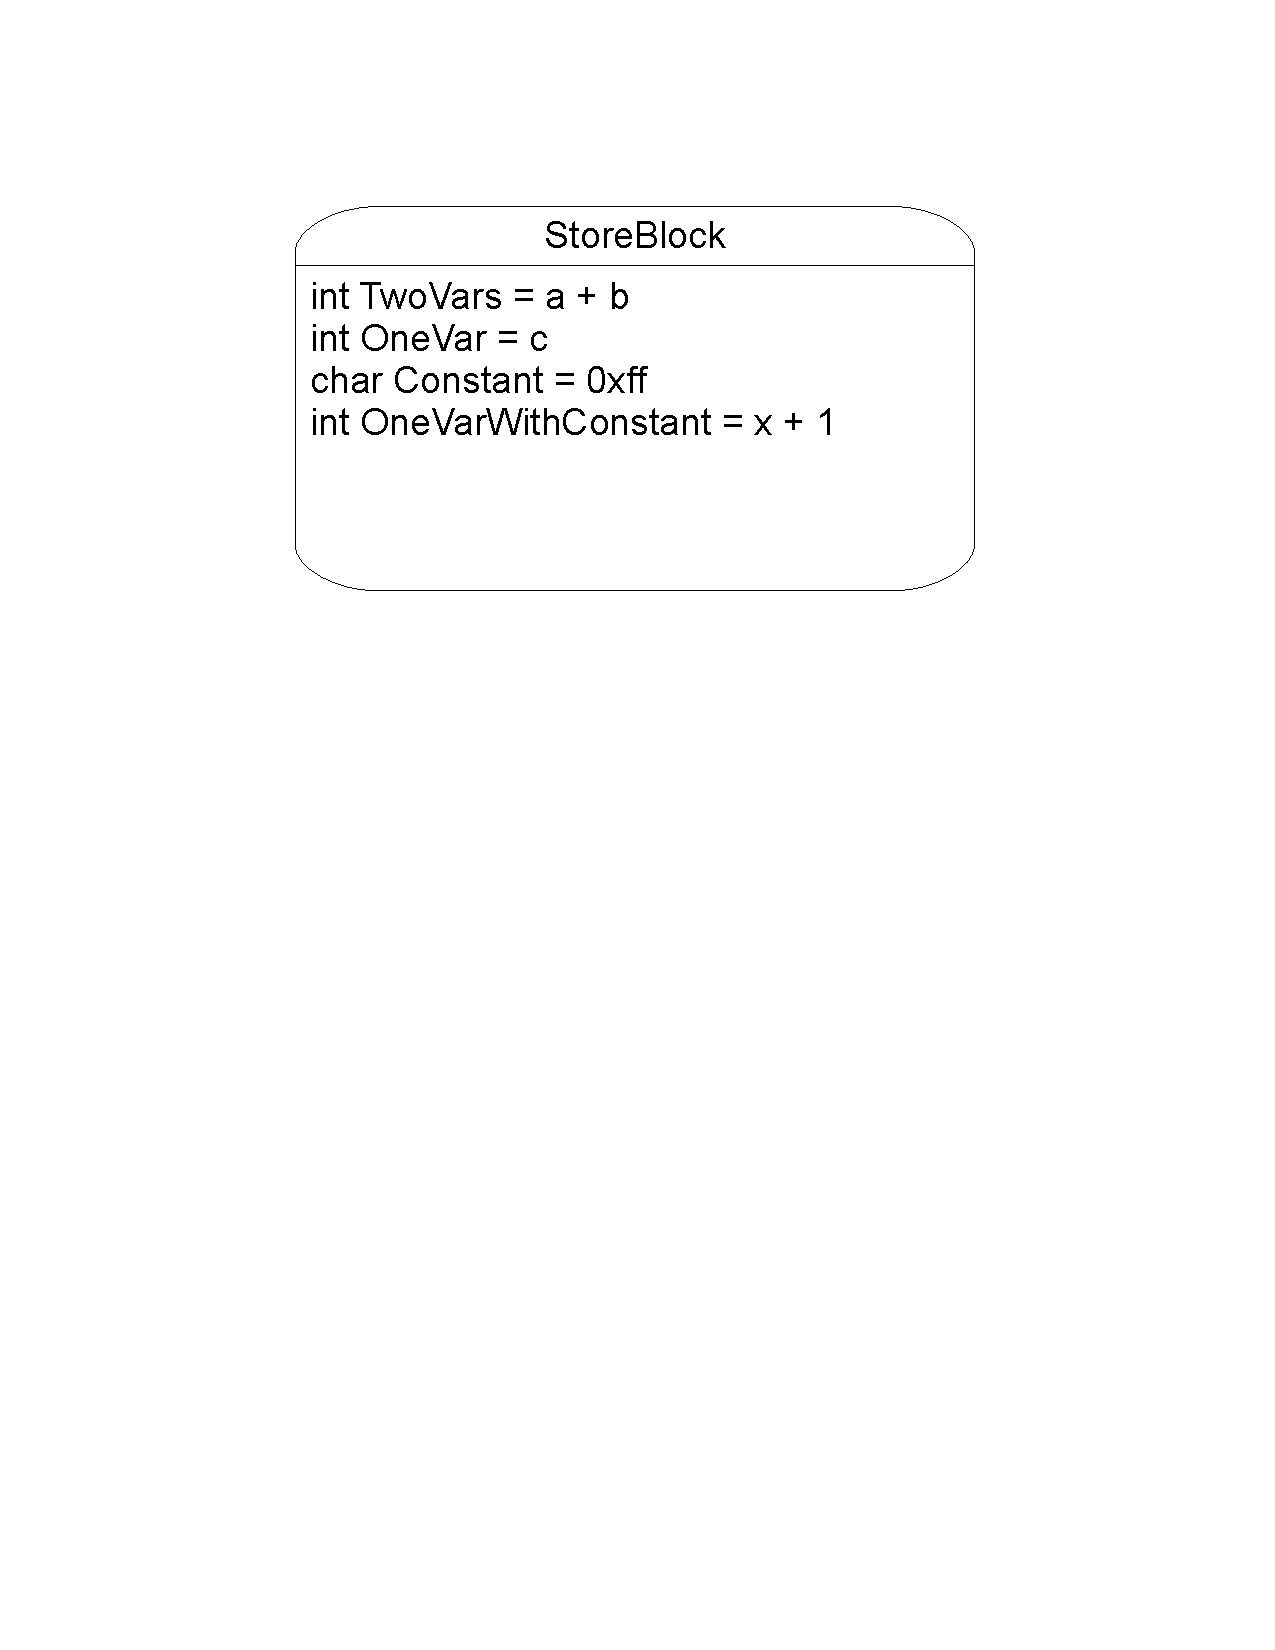
\includegraphics[trim= 20mm 175mm 20mm 10mm, clip, width=\imgmedium]{./images/state_storeblock.pdf}
    \caption{Example Of A Store Block As Implemented In PLCEdit}
    \label{fig:state_storeblock}
\end{figure}

In figure \ref{fig:state_storeblock} we see a store block represented as it would be drawn in the tool. Each line of a store block has the format shown in our abstract syntax. A line consists of a type (which in figure \ref{fig:state_storeblock} we have int, and char) an identifier, the equals symbol, and a value. A value can take the form of several expressions as shown in figure \ref{fig:state_storeblock}. Our abstract syntax also allows for many lines to occur in each StoreBlock. This basic design choice allows formulae to be computed much easier in sequence rather than have several blocks chained together to perform a set of operations.

Transitions in our system must start from an initial block object and must terminate at another block. Transitions must be mutually exclusive to be valid that is for all edges leaving the block conditions formed by expressions $E_1, E_2, E_3...E_n$: $\forall(i \neq j \rightarrow E_i \cap E_j = \emptyset)$. In addition given a set of conditions $E_1 \cup E_2 \cup E_3 \cup ... \cup E_n = \mathbb{U}$. In simpler terms all transition conditions must be mutually exclusive and must cover the entire space. It is an error in our language if you have a condition that can occur that is not explicitly described. It is valid to have a transition begin and terminate from the same block. 

\begin{figure}[htp]
    \centering
    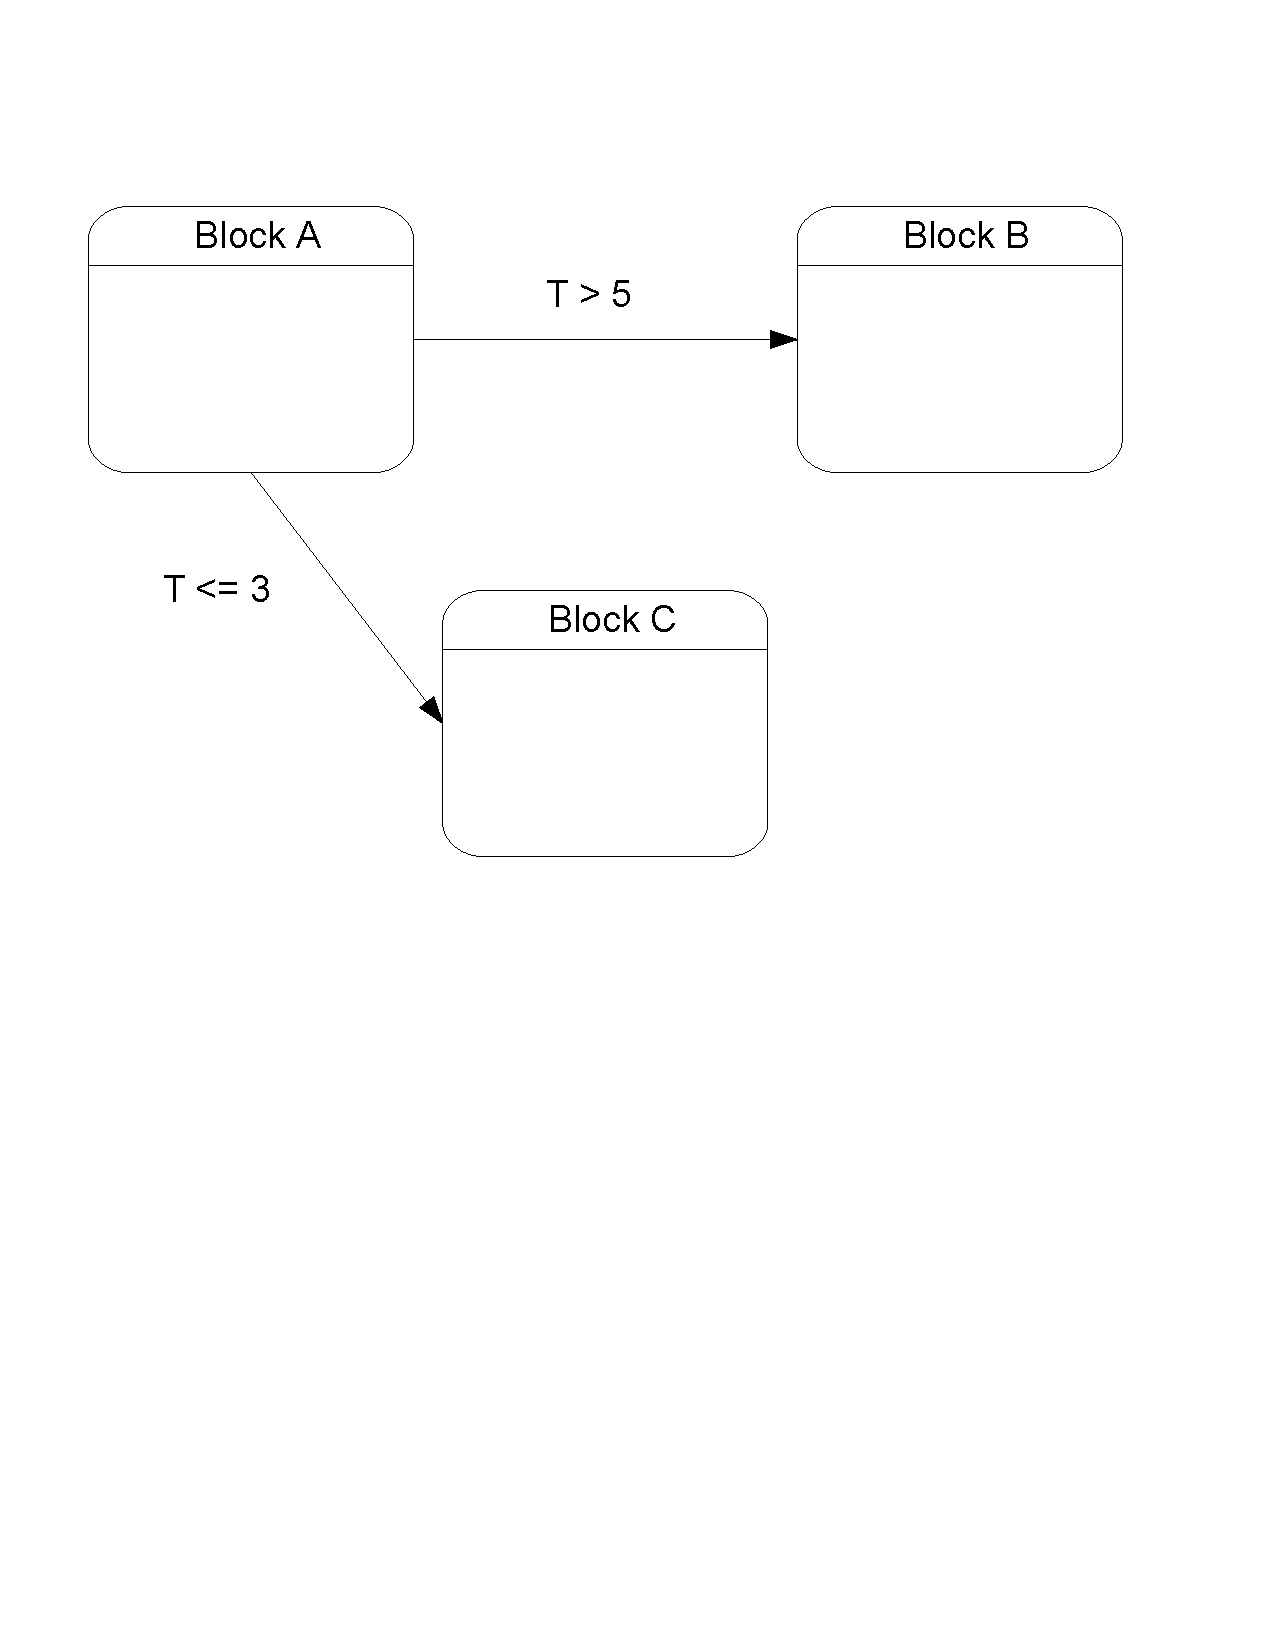
\includegraphics[trim= 10mm 130mm 20mm 10mm, clip, width=\imgmedium]{./images/state_transition.pdf}
    \caption{Example of Basic Transitions}
    \label{fig:state_transition}
\end{figure}





\clearpage

\newpage
%Implementation
\section{Implementation}
\subsection{GUI and IDE}
\subsubsection{Introduction}

The gui and ide are both implemented in JAVA with the JHotDraw 7.1 framework chosen as a basis. The gui was decided early on to function like other popular tools for drawing state charts such as Visio, IBM's Rational software, and Dia. All of these tools choose to be interactive in the drawing phase rather than compile a graph in post. The reason for enforcing interactive drawing is that this tool is design to simplify the original implementation of ladder logic, and building it on a textual graphical language will significantly hurt the primary goal of ease of use. Secondly JAVA was chosen for portability as it was simplier to test one deployment version than multiple ports for the short duration of this project.

The gui itself remains minimal %refer to figure
there is a simple toolbar in which objects can be selected from the pallete and drawn. Properties of an object are directly editable on the object itself %ref figure
instead of the original design of a seperate property palette. Again this design descision was chosen as it is simpler and more immediately understandable by the user.

%figure goes here

\paragraph{Using The Gui: Parts of the Gui}
\subparagraph{The tools pallate}
The tools pallate is were the user selects their tool to use on the canvas. Only one tool can be used at a time. All tools except for compile and simulation are selected on click. Compile and Simulaiton are immediately executed on click.
%TODO: Add simulation tool
The tools listed on the tool pallate are as shown in figure %create figure tool pallate
and have the functionality as follows
\begin{itemize}
\item \textbf{Selection Tool}: This tool allows you to select one or multiple objects. Or edit properties of objects. You can move the object around the canvas by first selecting the object with a single click, then clicking and draging the object to the desired location. Editing properties are accomplished by double clicking the property you would like to edit.
\item \textbf{Transition Tool}: This tool draws transitions between one block to another. Before you draw a transition you must have created the two blocks you wish to connect. To draw the transition you start by clicking and holding down the left mouse button over the starting block then dragging until the line snaps over the ending block. On release of the left mouse button a transition is formed and the two blocks are linked. For layout purposes you may also double click on a transition  line to add more anchors.
 %ref figure
\item \textbf{The StoreBlock Tool}: Store blocks are fundemental input blocks. You can use these blocks to perform calculations or update internal variables. To begin drawing a store block you first select this tool. Then you click on the canvas where you would like it to appear. Store blocks are auto-resizing objects thus the size is determined by the content. To edit each field in a store block you double click the parameter you wish to edit. If you wish to delete a line you can simple erase the identifier. If you wish to add a new line change the last identifier to something other than the default placeholder value. A new placeholder will be created as soon as you perform this action in order to allow you to add more lines.
\end{itemize}


\subsection{Data Flow}
..
\subsection{Structure}
..
\subsection{Compilation}
.. (maybe replaced by language section)

\newpage
%Correctness
\section{Correctness}
\subsection{The Graph Structure}
The graph structure chosen is simple directed graph in which the syntax and semantics are discussed in detail in sections \ref{sec:statechartsyn}, \ref{sec:statechartsem} respectively. To examine correctness we begin by looking at a basic atom and how it will be translated into the final code.

The simplest case is a diagram in which only the start node exists.
%add picture here.
In this simple example the following generated intermediate code \emphasize{IL} is created.

\begin{lstlisting}
// VARIABLE DECLARATIONS //
BLUID0:
//////////////////////////////////////
//        PROGRAM START             //
//////////////////////////////////////
goto EOF;

EOF:
\end{lstlisting}

In this simple atom of code we can see that there are no variables declared. We have a label inserted at the beginning of the start block so we can re-enter the start block if required. Because there is no other transition or block an automatic transition to \emphasize{EOF} is setup in order to terminate the program.




%the lower sections might be superceeded by the above.
\subsection{The IL}
\subsection{The Generated Code Sections}
\subsection{The Simulator}

\newpage
\chapter{Hardware}

\section{Platform}
\label{sec:hardwareplatform}

The initial hardware platform chosen for this project was the PIC18F452 however this project was designed from the ground up to allow for other hardware to be untilized with some effort from the hardware support team. The PIC18F452 was chosen due to its popularity in the industry and low cost.

In addition the PIC18F452 has the following features that are essential for PLC operation:

\begin{itemize}
\item 8 Digital inputs.
\item 8 Digital outputs.
\item 2 Ports.
\item Has support for C syntax.
\item Accessable hardware clock.
\item Onboard program memory.
\end{itemize}

These minimum specification have become the baseline for our hardware requirements. In order to utilize a different chip with our programming software the hardware support team will be required to implement a driver layer as described in seciton \ref{sec:hardwareframework}.

For real time operation hardware requirements on clock speed will become more critical execution of ``goto'' should occur as close as possible to constant time or O(1). Without the ability to execute ``goto'' in constant time delays between transitions become increasingly harder to predict and account for.

The specifications for the PIC18F452 are as follows:
\begin{itemize}
	\item CPU Frequency: 40Mhz
	\item Program Memory: 32K
	\item Data Memory: 1536 Bytes
	\item I/O Ports: 5
	\item Timers: 4
	\item 10-Bit A/D: 8 inputs channels
\end{itemize}

As the reader may observe the PIC18F452 exceeds our minimum requirements for hardware that will run our OS and software. In particular we currently do not include provisions to take inputs from our A/D channels which is a quite useful feature. This was done because we wanted seperate I/O modules to handle the inputs and outputs. Given more time on this project it would have been possible to fully utilize the onboard hardware.


\newpage
\section{Hardware Framework}
\label{sec:hardwareframework}

\subsection{Purpose}
The hardware framework allows different chips to be utilized with the same software code the same generated code from our software package ``PLCEdit'' as described in chapter \ref{ch:software}. Provided the hardware meets the minimum requirements defined by section \ref{sec:hardwareplatform}. The framework consists of a bunch of definitions which map the symbolic software references to hardware specific points. In addition the framework is also responsible for properly initializing the chip and performing any clean up operations once the chip finishes execution.


\subsection{Hardware Framework Overview}
TODO: include a diagram of the different hardware sections and how they fit together including the userland program.


TODO: Describe each section in detail.


\subsection{Chip Initialization} 
\textbf{File:} plcmcu.h

\textbf{Section:} Chip configuration 

\textbf{Description:} Sets configuration bits for the chip that cannot be done at runtime.

\textbf{Code:}
\\
\\
\begin{minipage}{\textwidth}
\begin{lstlisting}[frame=single]
...
#pragma config OSC = HSPLL //set occilator to HS-PLL
#pragma config OSCS = OFF //disable occilator switch
#pragma config PWRT = OFF //enable power on timer
#pragma config WDT = OFF //disable watchdog timer
#pragma config LVP = OFF //disable low power programming
...
\end{lstlisting}
\end{minipage}
\\
\\
\textbf{File:} plcmcu.c

\textbf{Routine:} init\_chip(void)

\textbf{Description:} Initializes any chip specific configuration bits that must be done at runtime.

\textbf{Code:}
\\
\\
\begin{minipage}{\textwidth}
\begin{lstlisting}[frame=single]
...
void init_chip(void)
{	
	TRISA = 0xFF; //set all portA to input
	TRISB = 0x00; //set all portB to output
}
...
\end{lstlisting}
\end{minipage}
\\
\\
\subsection{Hardware Specific Definitions}

Hardware specific definitions are reserved for defining specific characterists of the hardware to match up with the software. For example it may be necessary to define the input and output ports to a specific port on the chip itself.
\\
\\
\begin{minipage}{\textwidth}
\begin{lstlisting}[frame=single]
...
/* PORT specification */
#define PORTOUT PORTB
#define PORTIN PORTA
...
\end{lstlisting}
\end{minipage}
\\
\\
\subsection{Hardware Specific Implementations}

convenience calls from our software that access more complex operations may be required to be implimented directly into hardware. Our current software only requires that the routine for delaying the execution by a number of milliseconds is implimented. It is done as follows:

\textbf{File:}plcmcu.h
\\
\\
\begin{minipage}{\textwidth}
\begin{lstlisting}[frame=single]
/* CLOCK specification */
...

#define OCCILATOR 10000000 //our occilator in seconds
#define TCYTIME 1 //now many cycles / instruction 4 for non PLL 1 for PLL 

#define TCYTICK OCCILATOR / TCYTIME //how long per instruction tick
#define MSTIME 1000 //milliseconds to seconds

#define MSTCY TCYTICK / MSTIME //how many clocks in a ms (10000 for pll)

//crystal select block
#if (MSTCY >= 10000)
	#define DEFDELAY(timevalms) Delay10KTCYx(timevalms * (char) (MSTCY/10000))
#endif
#if (MSTCY >= 1000 && MSTCY void delayms(int time)
{
	DEFDELAY(time);
}< 10000)
	#define DEFDELAY(timevalms) Delay1KTCYx(timevalms * (char) (MSTCY/1000))
#endif
#if (MSTCY < 1000)
	#error "Unsupported OCCILATOR defined by hardware manufacturer please ensure crystal is faster than 1Mhz"
#endif

/* End CLOCK specification */

...
\end{lstlisting}
\end{minipage}
\\
\\
\textbf{File:} plcmcu.c
\\
\\
\begin{minipage}{\textwidth}
\begin{lstlisting}[frame=single]
...
void delayms(int time)
{
	DEFDELAY(time);
}
...
\end{lstlisting}
\end{minipage}
\\
\\
It is highly recommended to avoid macros where possible however the nature of the PIC18F452 required macros in order to prevent inaccurate delays caused by actually computations.

\newpage
\chapter{Summary}
\section{Contribution}

Things achieved in this thesis

PLCEdit IDE

PLCEdit compiler (tool)

PLCEdit simulator (tool)

Ladder Logic Analysis

Logic Control Chart: State Chart Language

Logic Control Chart: Semantics / Conventions / Operations


Driver for PIC18F452

Driver can be used as sample for creating an alternative system running on ATMega324P.. etc


MPLab Based tool-chain support with PLCEdit (PLCEdit generates MPLab compatabile compile files)


Things Accomplished Personal:

Understanding of Ladderlogic

Understanding of Various industrial applications for PLC's

Background information on PLC's and their current configuration

Background information on PLC and automation.


\section{Work To Be Continued}

TODO: FILL THIS OUT

\bibliographystyle{mcthesis}
\bibliography{main}
\appendix
\chapter{Appendix}
%appendix

\subsection*{Stepper Motor Examples}
\addcontentsline{toc}{subsection}{Stepper Motor Examples} 

\begin{figure}[h]
    \centering
    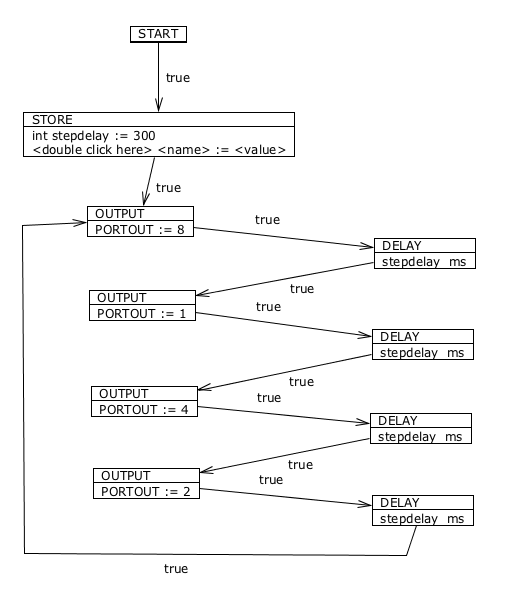
\includegraphics[width=0.7\textwidth]{./images/lcc_steppermotor.png}
    \caption{Running a Stepper Motor with \emphasize{\plcchart}}
    \label{fig:lcc_steppermotor}
\end{figure}

%

\begin{figure}[h]
    \centering
    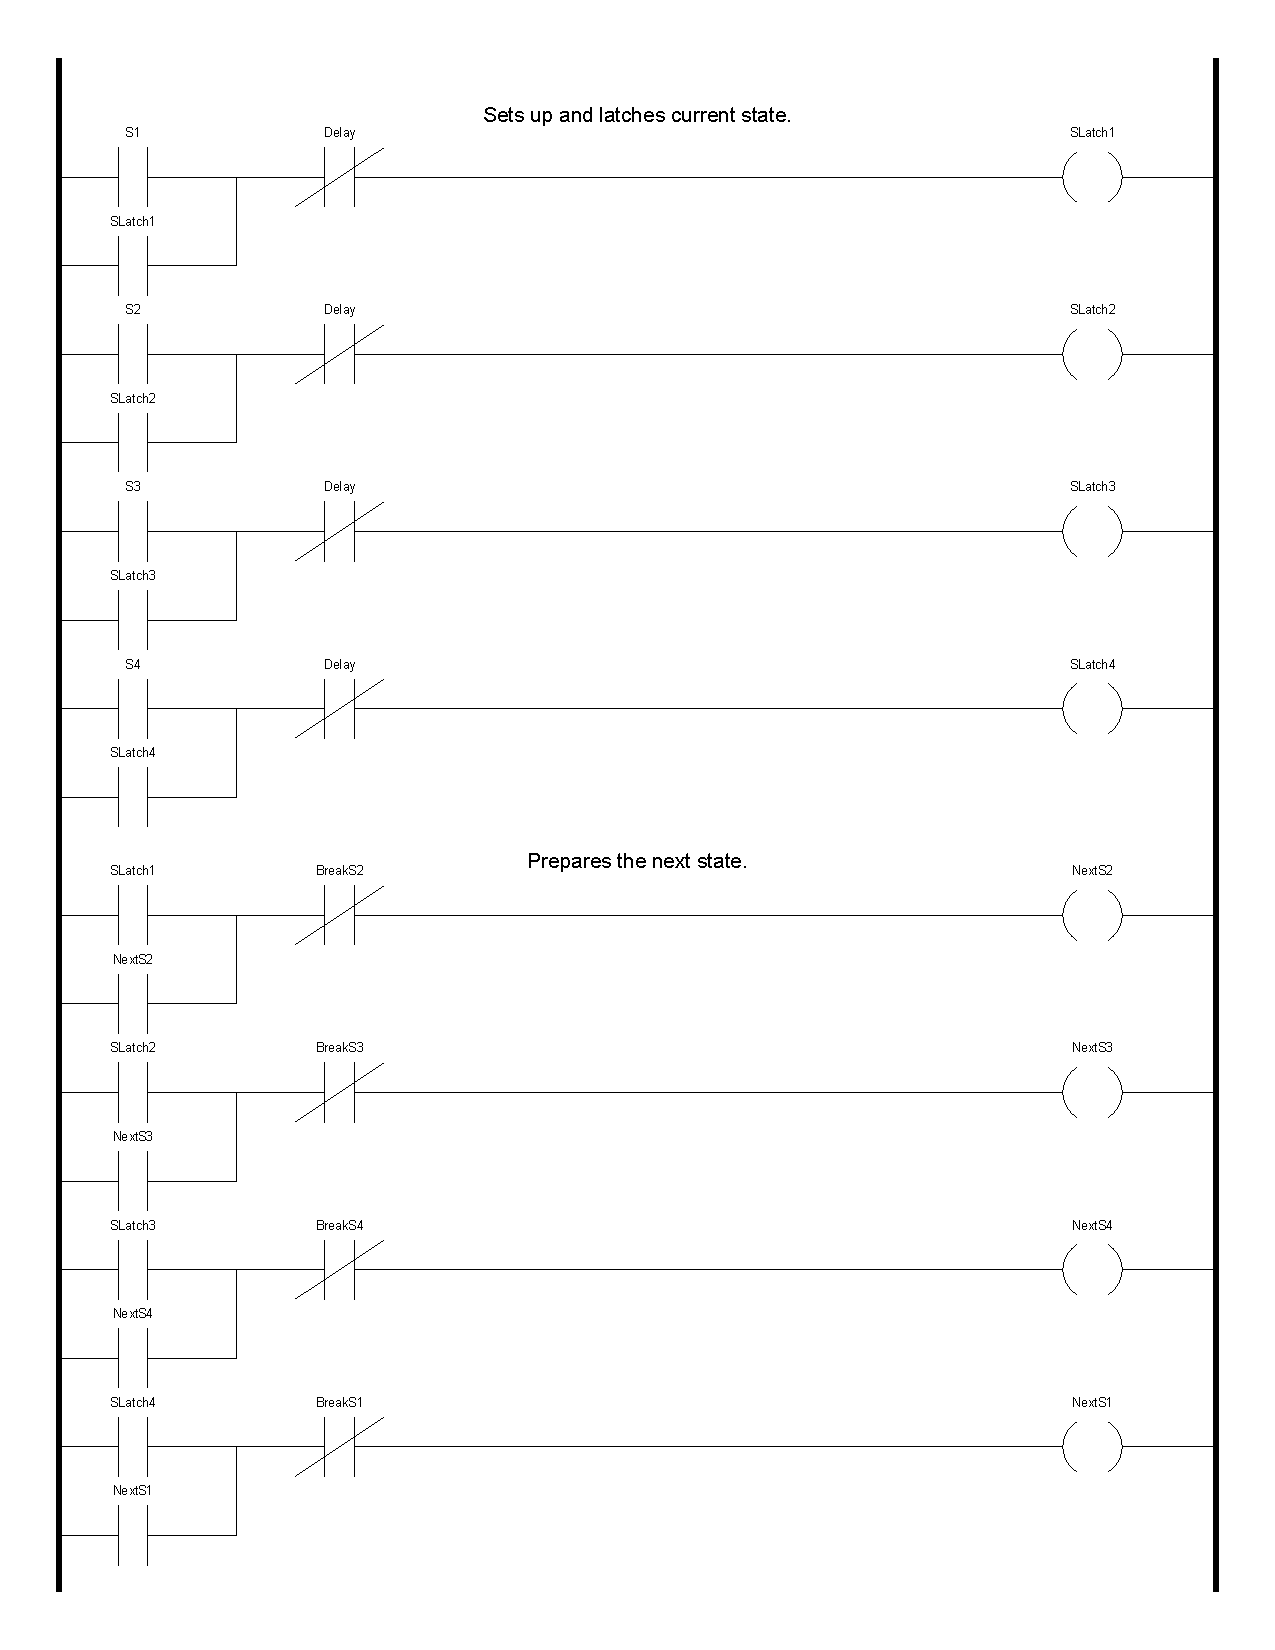
\includegraphics[width=0.7\textwidth]{./images/ladderlogic_stepper1.pdf}
    \caption{Running a Stepper Motor with \emphasize{Ladder Logic} part 1 of 3}
    \label{fig:ladderlogic_stepper1}
\end{figure}

\begin{figure}[h]
    \centering
    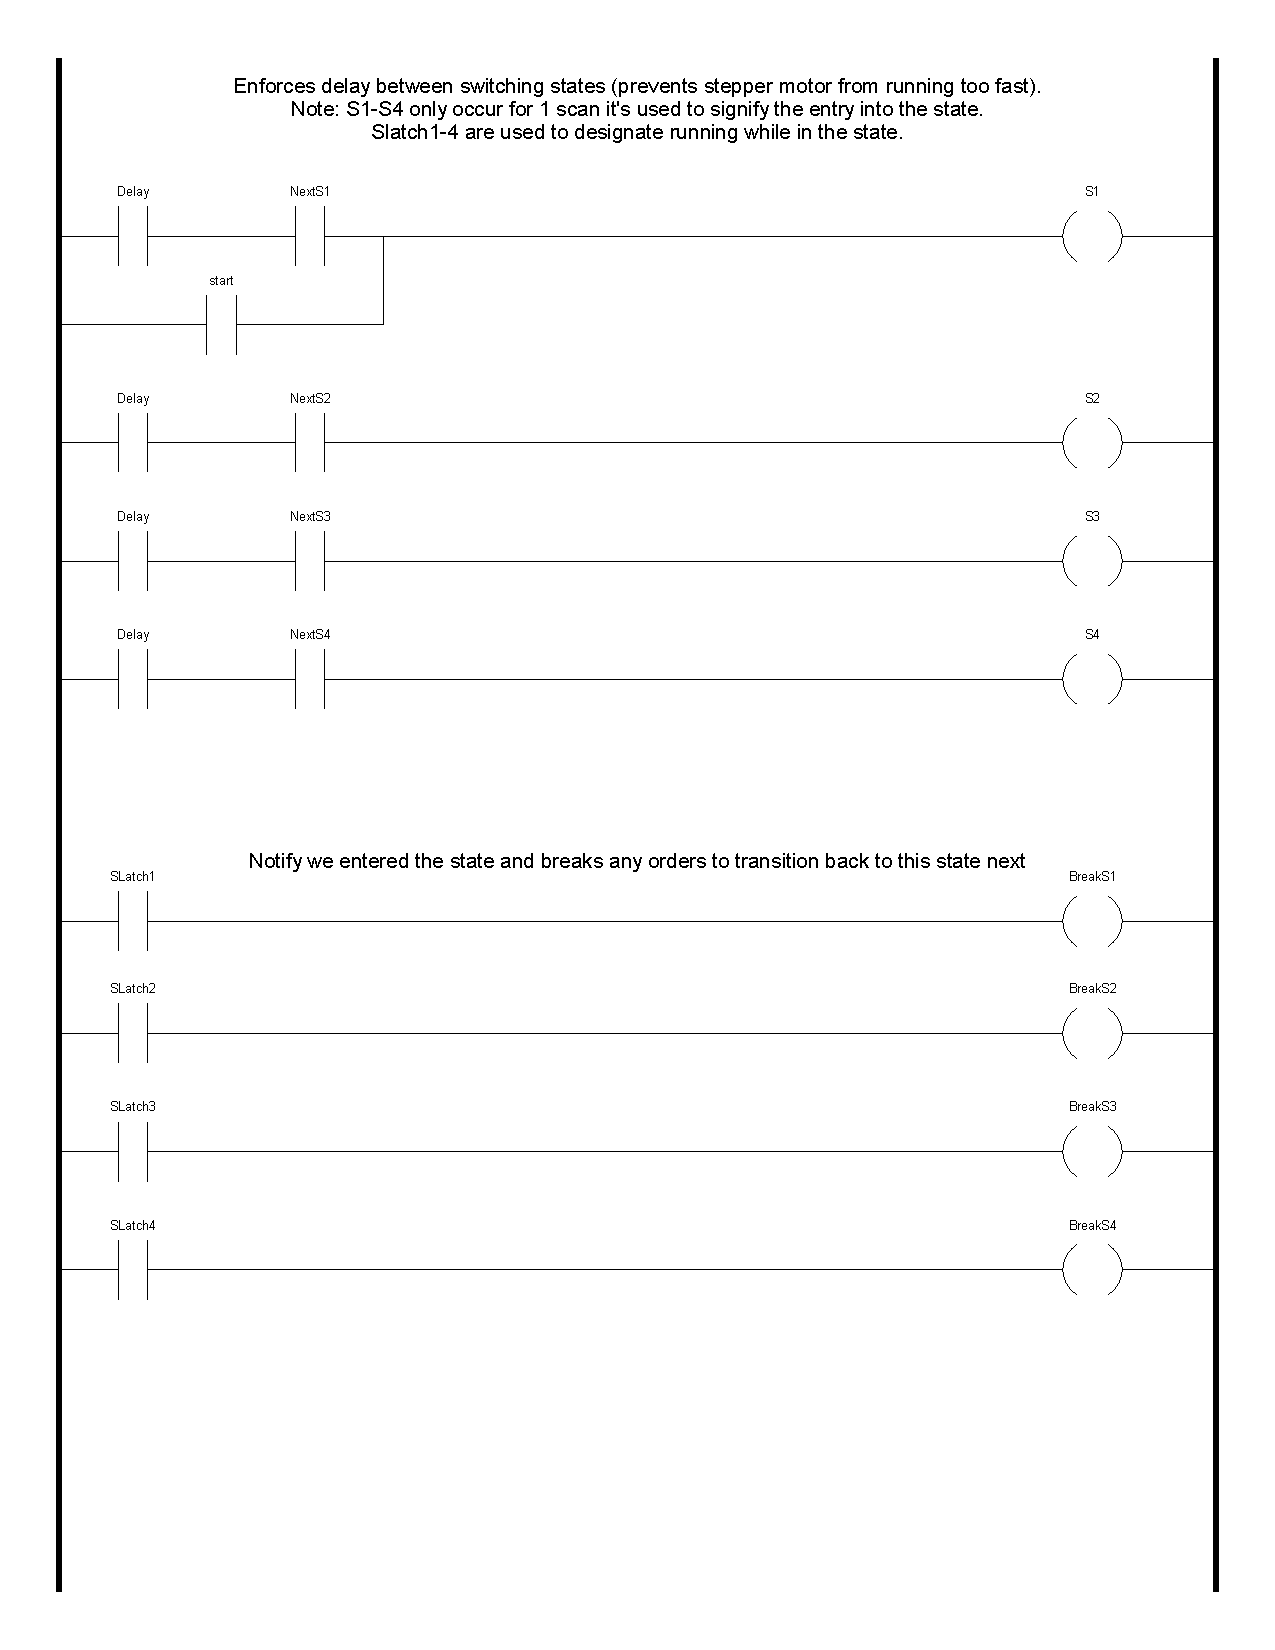
\includegraphics[width=0.7\textwidth]{./images/ladderlogic_stepper2.pdf}
    \caption{Running a Stepper Motor with \emphasize{Ladder Logic} part 2 of 3}
    \label{fig:ladderlogic_stepper1}
\end{figure}

\begin{figure}[h]
    \centering
    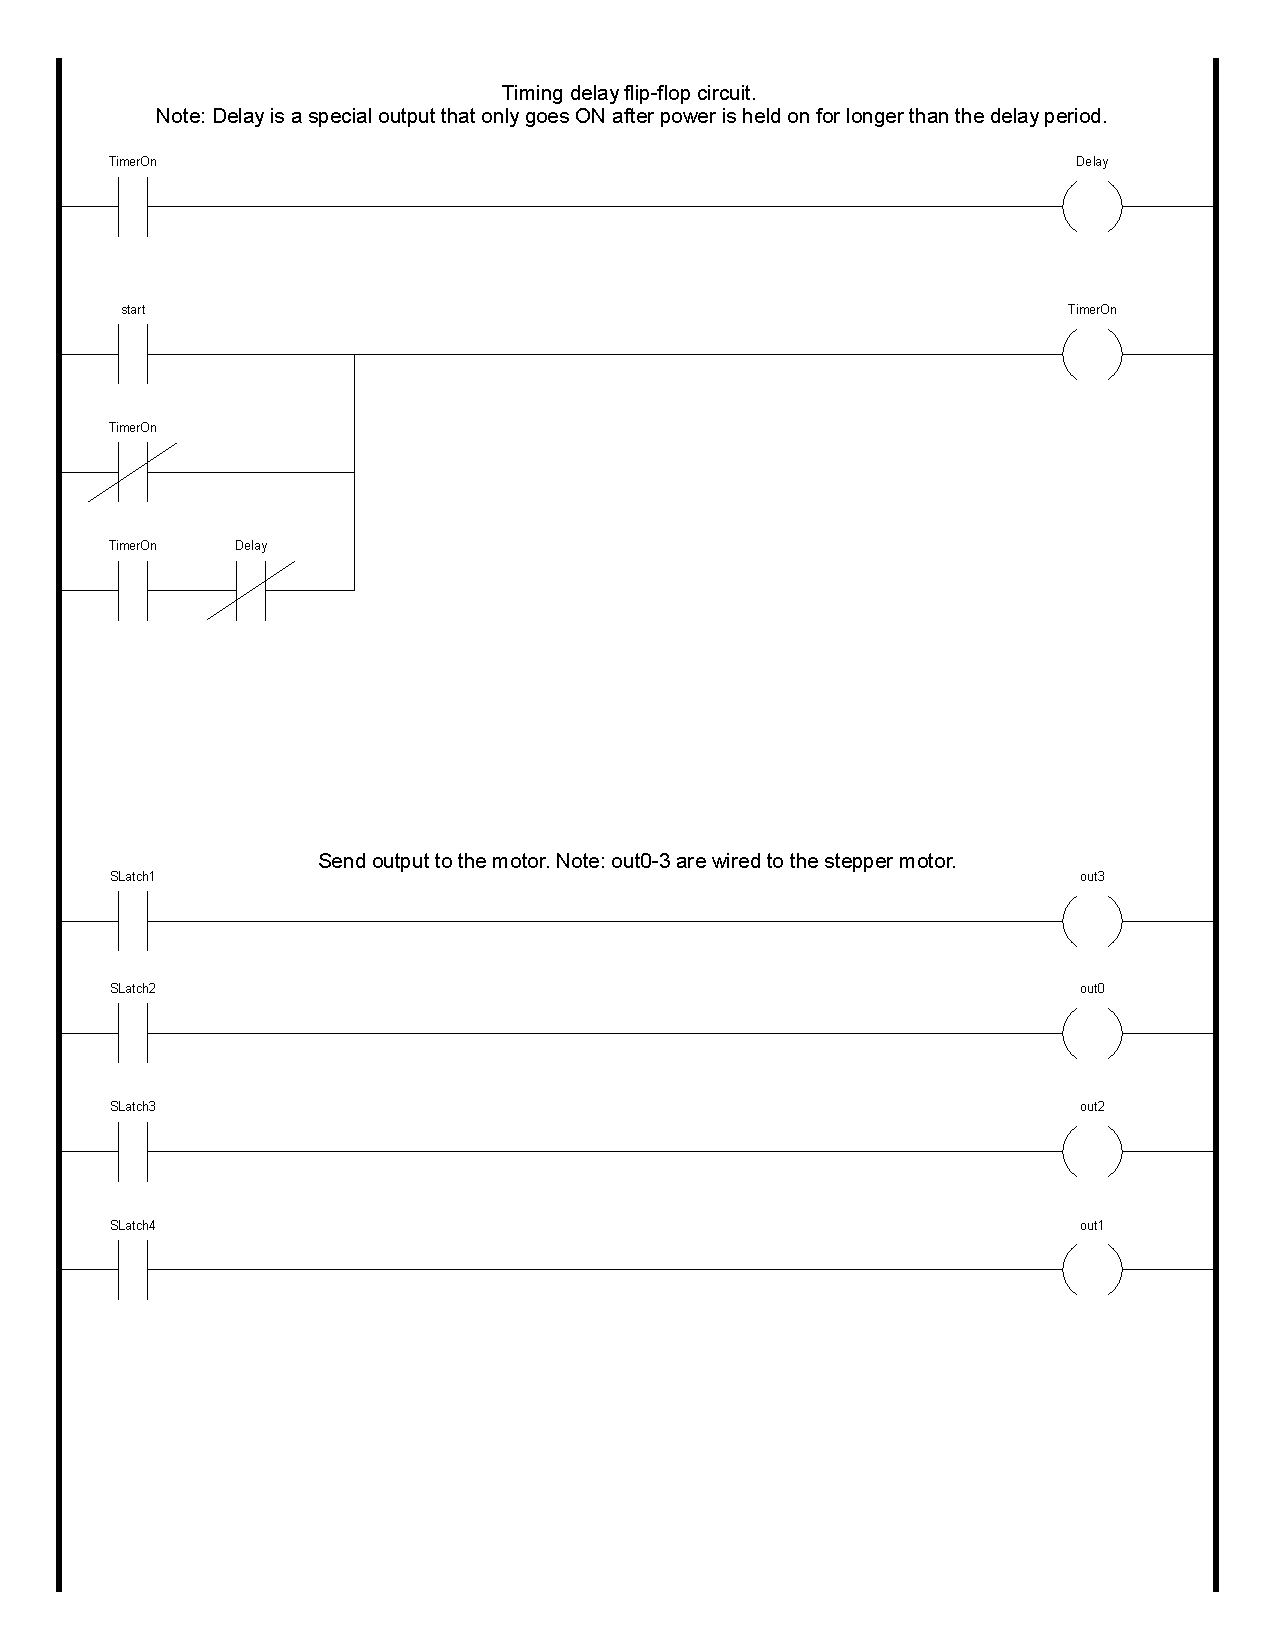
\includegraphics[width=0.7\textwidth]{./images/ladderlogic_stepper3.pdf}
    \caption{Running a Stepper Motor with \emphasize{Ladder Logic} part 3 of 3}
    \label{fig:ladderlogic_stepper1}
\end{figure}
\label{body end}
\end{document}
